%%%%%%%%%%%%%%%%%%%%%%%%%%%%%%%%%%%%%%%%%
% Stylish Article
% LaTeX Template
% Version 2.1 (1/10/15)
%
% This template has been downloaded from:
% http://www.LaTeXTemplates.com
%
% Original author:
% Mathias Legrand (legrand.mathias@gmail.com) 
% With extensive modifications by:
% Vel (vel@latextemplates.com)
%
% License:
% CC BY-NC-SA 3.0 (http://creativecommons.org/licenses/by-nc-sa/3.0/)
%
%%%%%%%%%%%%%%%%%%%%%%%%%%%%%%%%%%%%%%%%%

%----------------------------------------------------------------------------------------
%	PACKAGES AND OTHER DOCUMENT CONFIGURATIONS
%----------------------------------------------------------------------------------------

\documentclass[fleqn,24pt]{SelfArx} % Document font size and equations flushed left

\usepackage[english]{babel} % Specify a different language here - english by default

\usepackage [autostyle, english = american]{csquotes}
\MakeOuterQuote{"}
%----------------------------------------------------------------------------------------
%	COLUMNS
%----------------------------------------------------------------------------------------

\setlength{\columnsep}{0.55cm} % Distance between the two columns of text
\setlength{\fboxrule}{0.75pt} % Width of the border around the abstract

%----------------------------------------------------------------------------------------
%	COLORS
%----------------------------------------------------------------------------------------

\definecolor{color1}{RGB}{0,0,90} % Color of the article title and sections
\definecolor{color2}{RGB}{0,20,20} % Color of the boxes behind the abstract and headings

%----------------------------------------------------------------------------------------
%	HYPERLINKS
%----------------------------------------------------------------------------------------

\usepackage{hyperref} % Required for hyperlinks
\graphicspath{ {images/} }
\hypersetup{hidelinks,colorlinks,breaklinks=true,urlcolor=color2,citecolor=color1,linkcolor=color1,bookmarksopen=false,pdftitle={Title},pdfauthor={Author}}

%----------------------------------------------------------------------------------------
%	ARTICLE INFORMATION
%----------------------------------------------------------------------------------------

\JournalInfo{11 April 2016} % Journal information
\Archive{} % Additional notes (e.g. copyright, DOI, review/research article)

\PaperTitle{P2P Video Streaming with the Chord DHT} % Article title

\Authors{Alcuaz, Ito Franchilo Mikael\textsuperscript{1}
| Aziz, Shariq\textsuperscript{2}
| Ko, Mimi\textsuperscript{3}
| Musa, Abrar\textsuperscript{4}
} % Authors
\affiliation{\textsuperscript{1}\textit{y9u8, ialcuaz@alumni.ubc.ca}} % Author affiliation
\affiliation{\textsuperscript{2}\textit{i2u9a, shariqazz15@gmail.com}} % Author affiliation
\affiliation{\textsuperscript{3}\textit{o3d7, mimi@dbzmail.com}} % Author affiliation
\affiliation{\textsuperscript{4}\textit{i1u9a, abrar.musa.89@gmail.com}} % Author affiliation

\Keywords{} % Keywords - if you don't want any simply remove all the text between the curly brackets
\newcommand{\keywordname}{Keywords} % Defines the keywords heading name

%----------------------------------------------------------------------------------------
%	ABSTRACT
%----------------------------------------------------------------------------------------

\Abstract{
Media streaming refers to the constant delivery of time-ordered multimedia content from a server to a client. Naturally, such a system is centralized and demands a high bandwidth connection, which works more effectively for users on faster internet networks. A possible solution to this key shortcoming is found by de-centralizing the server-client model through the use of peer-to-peer (P2P) stream networking. This report discusses this group's implementation of a system which uses the Chord DHT -- a protocol which determines how to populate a distributed hash table. This protocol is used to correctly identify node placement in a ring overlay network, for joining and leaving cases, as well as to determine which nodes store which files, or parts of files. A user that wants to watch a video would then talk to the running system, of which relays back a video stream to be viewed on demand.     
}

%----------------------------------------------------------------------------------------

\begin{document}

\flushbottom % Makes all text pages the same height

\maketitle % Print the title and abstract box

\tableofcontents

\thispagestyle{empty} % Removes page numbering from the first page

%----------------------------------------------------------------------------------------
%	ARTICLE CONTENTS
%----------------------------------------------------------------------------------------

\section{Introduction} % The \section*{} command stops section numbering

A P2P implementation of a media streaming system alleviates some of the bandwidth requirements associated with media streaming. Usually the content is multicasted from a server to some number of clients which has requested the stream; YouTube makes use of this notion by deploying multiple content delivery networks (CDNs) which distribute the content by demand; the video content is streamed over a single connection. The key idea behind using P2P streaming is to make the system more scalable -- as the number of clients increase, so do the number of peers which can now make the data available to other clients who also requested the stream (similar to how P2P BitTorrent file sharing works).

A significant number of distributed hash table (DHT) models have been designed with the intent to be used in peer-to-peer (P2P) applications. A couple of the more popular prototypes include Pastry \cite{3} and Chord\cite{2}. DHT provides a useful infrastructure for P2P systems as it can locate data without the use of a centralized server. It is also scalable, distributes the content evenly, and routes among the nodes fairly quickly. The Chord DHT is specifically chosen as the overlay network for this system because it has a simple, standardized design, with well defined protocols to handle node behaviour.

This group's implementation focused on P2P streaming at the application level. As a brief overview, an overlay Chord system was constructed which handles node placement on a ring, file placement and replication, as well as maintenance of the ring structure as nodes enter/leave/fail. A client would then connect to the system and request to watch a given file, of which has been split over several different nodes. The nodes communicate among themselves to find the chunks of the video file (one node keeps track of the acquired and missing segments), and the video is then streamed back to the client in the form of serialized, encoded JSON messages. The VLC player then streams the video to the user as soon as a certain number of chunks become available (to minimize video buffering).

The rest of the report first discusses the design aspects of the system in depth, followed by implementation details, evaluation of the system as a whole, a discussion on what it succeeds on as well what it doesn't, and then finally the role that each team member played for the project.

\section{Design}

\subsection{DHT system structure/overlay and file storage}

\begin{figure}
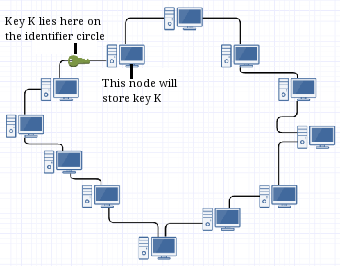
\includegraphics{Selection_152.png}
\caption{\label{family}The identifier circle and a storage of a key k into some node n.}
\label{1}
\end{figure}

Consistent hashing techniques is used to assign every node in the system an m-bit identifier. The SHA-1 hash on every node’s IP address/port combination is calculated, and this value is used as that node's unique identifier. For files, the SHA-1 hash of the file name will be calculated, which will be used to determine where the file will be stored, and that node is effectively the seeder of that file in the context of bit-torrent applications. The nodes themselves are going to be arranged in an identifier circle (see Fig. \ref{1}). To determine the positioning of a node in the circle, the distance between every other node's identifier (an SHA-1 hash of the IP address) and a particular node's identifier will be calculated to determine which node is the successor or predecessor on the circle.   

For some SHA-1 hash of a file k, it is stored at a specific node n if it is the very next node (clockwise) starting from the point where key k's identifier lies on the identifier circle (based on the calculated distance between the key k's hash and all the other nodes in the system), or on a node n if in the rare case of a hash collision where the SHA-1 hash of key k is equal to the identifier of n (giving a distance of zero). 

Maintaining only a single connection to the successor, while correct, would give a worst case linear runtime for searching a particular key, which is quite inefficient. To alleviate this problem, finger tables \cite{1} will be implemented at each node to keep track of node identifiers and their IP addresses. The ith entry in the table at some node n contains information about the node that succeeds n by at least $2^i - 1$. This means that the first entry is always the immediate successor of that node. The table steps along nodes exponentially so each node only ever needs to keep track of O(log($|$n$|$)) nodes, where n is the total number of nodes in our network (see Fig. \ref{2}).

Based on the above, where the max degree for each node is upper bounded by log($|$n$|$), a node, when faced with a query for a key k, will need only a lookup to the finger table to find a node which is closest to k’s identifier. Then it sends along the request to that node. The next node repeats the procedure recursively, and continues until it reaches a node which holds the key or has a successor which has that key-value pair. This reduces the lookup time to O(log$|$n$|$).

The node numbers on the circle will range from 0 to $2^m$ - 1. If a high enough m is chosen, 7 in our system, the probability of collisions is lessened and the system is more effectively load balanced. 

\begin{figure}[!htb]
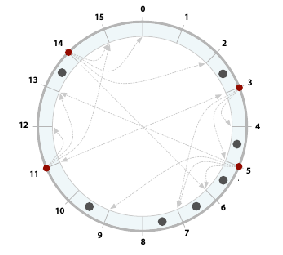
\includegraphics{Selection_155.png}
\caption{\label{family}Overlay network appearance with finger tables \cite{1}. Each node has a finger table which points to some other node. Only the finger tables of the red nodes are shown.}
\label{2}
\end{figure}

\subsection{Node joins and exits}

\begin{figure}[!htb]
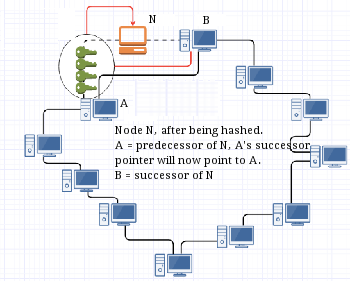
\includegraphics{Selection_153.png}
\caption{\label{family}Node entry case.}
\label{3}
\end{figure}

A joining node will have the SHA-1 hash of its IP calculated to identify a spot on the identifier circle. Once identified, the finger table of the predecessor will be updated accordingly to point to the new node (now its new successor), and recursively through all the finger tables of all the other nodes which had entries for the node that was moved over (now the successor of the new node) in the identifier circle (see Fig. \ref{3}). 

Specifically, to add or remove a node, two tasks should get done: updating all the routing tables that involve the node; and, transferring key responsibility from/to its new successor. These operations are known to cost time complexity $O(log|n|)^2$. Assume node B is node A's successor. To add C, the system updates the predecessor A's routing table according to C, and recursively do the same through the routing tables of all other nodes that have entries of B. C gains the responsibility for keys in the range of (a, c] which was previously part of B's key (a, b]. Now B is only responsible for keys in (c, b]. (see Fig. \ref{22}) Similarly, when C leaves or gets detected to be failed, all keys stored in C's routing table become reassigned to it's successor B. All associated routing tables remove C. The successor B now owns C's keys as well as its previous keys.

If a node fails/leaves all of its keys will be reassigned to it’s successor (see Fig. \ref{4}). The finger tables will also be updated recursively, removing every entry which previously held the exited node.

To detect failures, heartbeat messages will be sent from predecessor to successor; the successor expects a heartbeat from its predecessor every few seconds and if no reply was detected, then assume the node is lost and update the finger tables accordingly.

To deal with unexpected failures/a high churn rate and minimize the probability of data loss, every node in the circle will keep track of a subset arc of our identifier circle. For example, node n will maintain backups for node n+1, n+2 and n+3. So if in the near future, node n+2 fails, node n will be able to recover data (and send it to node n+4 since it’s the next best candidate for storing all of n+3’s keys). This window of backups shall be maintained for every node in our network, allowing for quick recoveries. The replication factor r  is decided beforehand as possibly an argument to the go program, but this will generate a certain number of backups that should ideally scale to O(log$|$n$|$).

\begin{figure}[!htb]
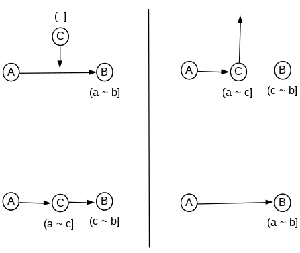
\includegraphics{figure1.png}
\caption{\label{family} Left: key transfer with new node. Right: key transfer with removed node.
}
\label{22}
\end{figure}

\subsection{Ring maintenance}

Every participating node is a member of a ring. The node has links to a successor node (whose key is next highest) and a predecessor (whose key is closest past). The successor is also defined as the smallest key entry stored in each routing table. Chord ring topology is defined by the successor pointer. To maintain this topology, the system is required to have exactly one ring and all members in the ring in right order \cite{4}.

Before any addition or removal of nodes proceeds, the ring's member relation is redefined. When the previous example of adding a node is about to occur, node C first asks the predecessor A for A's current successor key. The returning key is of node B, which becomes C's successor; and C becomes B's predecessor (represented as dashed line in Fig. \ref{55}). Until A notices that B now points to a different predecessor than itself, B has two members believing that they are the successor. 

\begin{figure}[!htb]
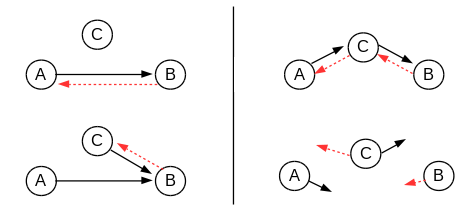
\includegraphics{figure3.png}
\caption{\label{family}Left: adding node C to the ring. Right: removing node C from the ring.}
\label{55}
\end{figure}

As seen in Fig. \ref{56}, the ring seems maintain with an appendage cause by C. However it does not circulate properly because A's idea of its successor B and B's idea of its predecessor C do not agree. High node churn rates in particular make this part troublesome. The original Chord paper \cite{2} suggests a protocol where each node periodically checks if its successor is still alive and updates their finger table accordingly (see Fig. \ref{5}). This protocol has been implemented into the system, and this detection runs in the background using heartbeat messages (to test for abrupt disconnections, as explained in section 2.2).

\begin{figure}[!htb]
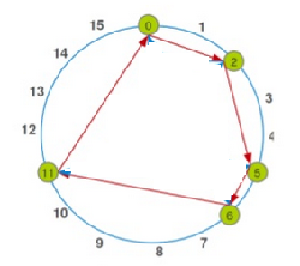
\includegraphics{stabilize1.png}
\caption{\label{family}Handling peer churn. The correct successor is the first node that is found to be alive by traversing in the clockwise direction (red arrows).}
\label{5}
\end{figure} 

\begin{figure}[!htb]
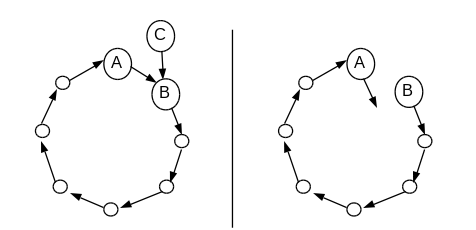
\includegraphics{figure5.png}
\caption{\label{family}Left: adding node C to the ring. Right: removing node C from the ring.}
\label{56}
\end{figure}

Every member pings the node whose key is locally stored as its processor and ask for its predecessor. In case the returned predecessor key does not agree with itself, the node redirect its successor pointer to the returned predecessor. Then the new predecessor will set its predecessor pointer to this node and the ring is repaired. For example, node A in Figure 5 asks node B for what B's predecessor is and B returns node C. Since B's predecessor is not A itself, A adopts B's predecessor C as new successor. For A, C is a rational choice for its successor because C clearly has larger key than A's – otherwise C could not have been A's former successor B's predecessor – and smaller than B's because B is C's successor. Thus after C sets A as its predecessor successfully, it continues to update routing tables and key responsibilities as appropriate. Since the paper does not provide much more details, the member is set to send two arbitrary messages expecting one back, as described on the page 3 of the proposal.

An obvious weakness of this method, also mentioned in the Chord paper, is that it cannot handle concurrent joins. If more than two nodes C, D join between two members A, B (Figure 7) before the periodic heartbeat incorporates at least one node into the ring, B eventually sets its predecessor pointer to the later added D. Once A has been stabilized, it recognizes D as its successor and transfers proper key responsibility to D. C becomes not reachable from other members. Although this does not violate P. Zave's conditions for a “valid” overlay structure (i.e., exactly one ring and ordered), it is incorrect in terms of key responsibility. After the stabilization B becomes responsible for keys (D, B]. Thus a key between (D, C) will belong to B. However C is a live node that deserves to own the key in the range. The stabilization protocol and the successor list together resolve most of the cases regarding member changes in the ring. 

\subsection{Media streaming and delivery}

Some nodes have stored in them a multimedia file, such as an MPEG file, which is effectively synonymous with seeders in bit-torrent applications. When a client wants to stream a video from its peers, it will do a lookup on the finger table to obtain the id of the node that has the file. Once a node is obtained, a lookup on the finger table of that node for another node that has the video file will be done. In doing so, once a certain number of nodes for the file is obtained, a stream to the video is initialized, which will be done in terms of a sequence of frames. 

A queue to store a list of all the frames of the video will be used and will keep asking the connected nodes for the frames in sequence. In the case where a later frame is obtained sooner than an earlier frame, the frame is stored in a buffer and the playback of the frames will occur only once an ordered sequence has been obtained. 

In the case where nodes that were sending frames die or leave the network, the frame requests are redistributed across other available and connected nodes. In the exceptional case where all nodes except for the client are lost, lookups on the finger table will be performed for alive nodes that contain the file, and once at least one alive node is obtained, send the node the frame request again. This assumes consistency across all the nodes in terms of finger tables.

\section{Implementation Details}

\subsection{Chord DHT Overlay Network}

The structure of the system was implemented using one Go file -- src/customChord/customChord.go. No external libraries were used. A node connects to a system given at least one ip:port combination of a running node, or in the case of boot up, a node starts up a UDP listener and awaits for incoming join requests. Note that all nodes in the system listen for UDP packets on a given port, and as such, any node in the system can be used as an entry point. The nodes communicate amongst themselves, again, using UDP packets (the message is first encoded in JSON format). Once a node receives a UDP packet, it will unmarshall it into an interface object, and according to the message, will handle it accordingly. The message can be of several types, including join requests, file placement, or the result of a previous join request (the nodes use this information to place joining/failed nodes along the identifier circle), etc. The finger tables and file relation tables are implemented using standard Go maps. Since each node interacts with its own finger/file table after a UDP read, there is no concurrency in the system.

\subsection{Streaming Implementation}

The streaming portion of this system made use of FFMPEG and HTTP external libraries to properly encode/decode video files and split them among the nodes. A given file is split into a sequence of JSON encodings, together all of which completely describes a given MP4 file. VLC can easily decode a given sequence into a playable video file. To initiate a stream, a streaming server and client communicates via RPC to any running node, who would then find the required video segments from the other nodes in the system. 

\section{Evaluation}

\subsection{Chord DHT Overlay Network and ShiViz Integration}

The system was tested against a limited number of nodes for correctness, on a local network. As such, it is assumed that no packets are lost in node-node communication. Correctness was evaluated on the basis of the contents of the finger tables after joins and failures. It was also tested if files get saved at the correct locations along the ring. Since each node is effectively both a client and server, the addition of GoVector logs was straight forward, as an event is produced when a node (in its main thread, since the system has no concurrency apart from heartbeat messages) either reads a UDP packet, sends a UDP packet, or responds via RPC to a stream request. Since there is a fair amount of communication required, the ShiViz diagrams are heavily populated, but one can then track the messages that are sent and received.

Note that there are currently some issues regarding the ShiViz integration, and so the logs are not properly outputted. This issue will be fixed in time for the demo.

\subsection{Streaming}

The system was tested using a sample MP4 file which was split into a file of JSON encodings (of which are replicated across some number of nodes in a system). Correctness is then to just simply see if the file correctly plays, and in order, through VLC. There should be no loss of quality as all the testing was done locally, and so packets should not have been lost. 

\section{Limitations}

A key limitation on our system is the fact that we are using UDP packets as a means for communication. This would be fine if we intended to keep the project at a local level, but would present complications if the project gets deployed at a later stage, as we'd have to account for lost packets between point A to B. A more standardized way would have been to use RTP transmission protocols but there wasn't enough time to experiment with it. 

\section{Discussion and Work Allocation}

The project was quite ambitious in scope, and it would've been very beneficial on our end if we got a bit more time so that we could polish it up and handle more edge cases, as well as deployment onto a web server. 

We allocated the tasks into two main parts: streaming and the Chord structure implementation. Abrar (ilu9a) and Mimi (o3d7) both handled the streaming aspect, whilst Ito (y9u8) handled parts of the main structure implementation, as well as ShiViz integration, and Shariq (i2u9a) coded both the streaming and main structure functionality.


\section{Conclusion}

A possible solution to the drawback of the centralized client-server model in media streaming can be found through the use of a P2P network. This is achieved by sharing the bandwidth requirements across several disjoint nodes which serve to forward the data stream among themselves, not over one singular connection. Such a system is complicated to build however, and gives rise to its own set of disadvantages. Peer churn in particular, remains a significant challenge and one that is still not adequately addressed with most current P2P implementations.

\phantomsection
\bibliographystyle{unsrt}
\bibliography{sample}

%------------------------------------------------

\end{document}